\setchapterpreamble[u]{\margintoc}
\chapter{Flower Calculus}
\labch{flowers}

\epigraph{In a certain flower garden, each flower was either red, yellow, or
blue, and all three colors were represented. A statistician once visited the
garden and made the observation that whatever three flowers you picked, at least
one of them was bound to be red. A second statistician visited the garden and
made the observation that whatever three flowers you picked, at least one was
bound to be yellow. Two logic students heard about this and got into an
argument. The first student said: "It therefore follows that whatever three
flowers you pick, at least one is bound to be blue, doesn't it?" The second
student said: "Of course not!". Which student was right, and why?
}{\textbf{Raymond Smullyan}, \textit{The Flower Garden}, 1985}

We introduce the \emph{flower calculus}, a novel proof system for intuitionistic
predicate logic based on syntactic objects called \emph{flowers}. We start by
explaining how flowers stem from considerations in graphical logic, and more
specifically from an intuitionistic variant of the \emph{existential graphs} of
C. S. Peirce proposed by A. Oostra \sidecite[12.5em]{oostra_graficos_2010}. Then
we present our inductive syntax for flowers, reminiscent at the same time of the
nested sequents of deep inference proof theory, and the geometric/coherent
formulas of categorical logic. A salient feature of our calculus inherited from
EG, is that it is \emph{fully iconic}: it dispenses completely with the
traditional notion of symbolic formula, operating instead as a rewriting system
on flowers containing only atomic predicates. We also propose a notion of proof
geared towards analyticity results à la Gentzen, suggesting new rules absent
from other works on intuitionistic EG. This allows us to prove admissibility
theorems for many rules, including Peirce's deletion rule which is a variant of
Gentzen's cut rule. These results are obtained as a consequence of our soundness
and completeness proofs with respect to Kripke semantics, in the spirit of the
\emph{normalization-by-evaluation} technique \sidecite{NbE}. Furthermore, the
kernel of rules targetted by completeness is fully invertible, a desirable
property in both automated and interactive proof search. This is illustrated by
our implementation of the Flower Prover, an early prototype of GUI for ITP that
uses the rules of the flower calculus both for direct manipulation of flowers in
its frontend, and automated simplification of goals in its backend.

The chapter is organized as follows: in \refsec{IEG}, we retrace the origin of
Oostra's syntax for intuitionistic EG (hereafter ``IEG'') as a natural
generalization of the \emph{scroll}, an icon for implication introduced by
Peirce that inspired the very creation of EG. In \refsec{Flowers}, we explain
how flowers are really just a fun and metaphorical way to draw IEG, and proceed
to give them an inductive, multiset-based syntax as in \refsec{multisets}. In
\refsec{Calculus}, we introduce the full set of inference rules of the flower
calculus as well as our notion of proof, and prove a few syntactic properties,
including a deduction theorem. In \refsec{Semantics}, we give a direct Kripke
semantics to flowers, avoiding the need for translations to and from formulas.
In \refsec{Soundness}, we show that the rules of the flower calculus are valid
with respect to our Kripke semantics, and in \refsec{Completeness} we identify a
complete fragment of the system where all rules are both \emph{analytic} and
\emph{invertible}. This entails the admissibility of all rules outside of this
fragment, and as a consequence the analyticity of the system. We exploit these
properties in \refsec{flowers-search} by describing an algorithm for fully
automated proof search in the propositional fragment, that we conjecture to be
complete. Then in \refsec{flowers-prover} we give an overview of the Flower
Prover, a prototype of GUI in the Proof-by-Action paradigm whose actions map
directly to the rules of the flower calculus, and which integrates nicely with
our search procedure. In \refsec{flowers-curryhoward}, we briefly sketch some
ideas for a Curry-Howard correspondence, where flowers and actions for
manipulating them are identified respectively with \emph{normal} and
\emph{neutral} terms of the $\lambda$-calculus. We conclude in
\refsec{Conclusion} by a comparison with some related works, and a discussion of
future works and applications that we envision.

% \section{Introduction}

% \subsection{Interactive proof building}

% Given a sufficiently expressive logic, the problem of finding a formal proof of
% a given statement in that logic is notoriously hard. Not only because of
% undecidability, but because proof calculi are very rigid, and expose too many
% details compared to the informal proofs that mathematicians are used to write.

% One way to tackle this limitation is to design search procedures for interesting
% fragments of the logic under consideration. This is the approach undertaken by
% automated theorem provers such as SMT solvers, or more specialized decision
% procedures such as Coq's \texttt{lia} tactic for linear integer arithmetic.
% Still, large-scale proofs of complex theorems currently require a human in the
% loop to provide the overall structure of arguments, but also of the theories
% built up from definitions and lemmas.

% This is where proof assistants come in, by providing a set of tools to make the
% whole process of formalizing mathematical developments easier. This includes
% languages to specify definitions and statements conveniently, but also
% interfaces to build proofs interactively without having to fill in all the
% details. The dominant paradigm for these interfaces is that of \emph{tactic
% languages} \sidecite{doi:10.1098/rsta.1984.0067}: the user is exposed with a set of
% \emph{goals} that remain to be proved, also called the \emph{proof state}, and
% modifies these goals through textual commands called \emph{tactics} until there
% is no goal left. This is currently what is implemented in mainstream proof
% assistants such as Coq \sidecite{the_coq_development_team_2022_7313584}, Isabelle
% \sidecite{nipkow2002isabelle} and Lean \sidecite{10.1007/978-3-030-79876-5_37}.

% \subsection{Graphical interfaces}

% In recent years, there have been many efforts to replace or complement textual
% tactic languages with modern \emph{graphical user interfaces} \sidecite{PbP}
% \sidecite{langbacka-tkwinhol-1995} \sidecite{Chaudhuri2013} \sidecite{edukera}
% \sidecite{zhan-design-2019} \sidecite{ayers_graphical_2021}. The hope is to make proof
% assistants more intuitive and accessible to beginners and non-specialists, but
% also to some extent more productive and ergonomic for experts. 

% The initial motivation for this work was to design a proof calculus well-suited
% to \emph{direct manipulation} in such a graphical setting. The idea is that the
% user should be able to interact directly with the graphical representation of
% the proof state, using a pointing device such as a mouse or fingers on a touch
% screen. In previous work \sidecite{10.1145/3497775.3503692}, we proposed a way to
% synthesize complex logical inferences through \emph{drag-and-drop} actions
% between two items of the current goal. Since goals are represented as
% \emph{sequents} $\Gamma \vdash C$, the items involved were traditional logical
% formulas, either two hypotheses in $\Gamma$ or one hypothesis and the conclusion
% $C$.

% \subsection{Non-symbolic reasoning}

% In this work we show that sequents and formulas built from binary connectives
% and quantifiers are unnecessary for representing the proof state. We speculate
% that they actually get in the way of a natural flow of information in the proof,
% and do not capture accurately the way mathematicians organise hypotheses and
% conclusions in their reasoning. A similar argument has been made by E. Ayers in
% his thesis \sidecite{ayers_thesis}, where his solution is to design a nested goal
% data structure called \texttt{Box} on which reasoning can be performed directly
% without relying on formulas.

% % TODO: reference precise chapter of Ayers thesis

% We introduce a closely related structure for goals, but inspired instead by an
% early invention in the history of graphical logic: the \emph{existential graphs}
% of C. S. Peirce \sidecite{Roberts+1973} (thereafter written ``EG'').
% We noticed that our structure could be drawn and manipulated metaphorically in
% the form of nested \emph{flowers}, and thus decided to name \emph{flower
% calculus} the proof system that we built around it. Our focus in this work will
% be to study the fundamental properties of the flower calculus, mainly through
% the lens of modern structural proof theory. We only hint at some ways the
% calculus could be used as a foundation for a graphical theorem proving
% interface, and leave a more systematic proposal for future work.


\todo{Make all usages of notations consistent with \reftab{letters}}


\section{Intuitionistic existential graphs}\labsec{IEG}

\paragraph{The Scroll}

In \refsec{alpha}, we presented the syntax of existential graphs (EG) as
stemming from two fundamental icons: the \emph{sheet of assertions} ($\SA$),
with its ability to represent the conjunction of assertions through
\emph{juxtaposition}, and \emph{cuts} in $\SA$ that signify the denial or
negation of assertions. However as noted in \refremark{eg-entitative}, the first
interpretation of juxtaposition proposed by Peirce was that of
\emph{disjunction}, in his system of \emph{entitative graphs}. According to him,
the illative transformations of EG are a necessary consequence of the
\emph{conjunctive} interpretation of juxtaposition, as witnessed by the
following excerpt \cite[p.~533]{peirce_prolegomena_1906}:

\begin{quote}
If you carefully examine the above conventions, you will find that they are
simply the development, and excepting in their insignificant details, the
inevitable result of the development of the one convention that if any Graph, A,
asserts one state of things to be real and if another graph, B, asserts the same
of another state of things, then AB, which results from setting both A and B
upon the sheet, shall assert that both states of things are real.
\end{quote}

He goes on to notice:

\begin{quote}
   This was not the case with my first system of Graphs, described in Vol. VII
of The Monist, which I now call Entitative Graphs. But I was forced to this
principle by a series of considerations which ultimately arrayed themselves into
an exact logical deduction of all the features of Existential Graphs.
\end{quote}

Thus the conjunctive reading of juxtaposition itself stemmed from ``a series of
considerations'' that ``forced'' Peirce to adopt it. While in this article he
does not give the full ``exact logical deduction of all the features of
Existential Graphs'', he exposes in some details the initial and determining
insight that kickstarted the whole development: the discovery of the icon called
the \emph{scroll}. Again, I will let Peirce speak for
himself \cite[pp.~533--534]{peirce_prolegomena_1906}:

\begin{quote}
  Accordingly, since logic has primarily in view argument, and since the
conclusiveness of an argument can never be weakened by adding to the premisses
or by subtracting from the conclusion, I thought I ought to take the general
form of argument as the basal form of composition of signs in my
diagrammatization; and this necessarily took the form of a ``scroll'', that is
[...] a curved line without contrary flexure and returning into itself after
once crossing itself, and thus forming an outer and an inner ``close''.
\end{quote}

\begin{marginfigure}
  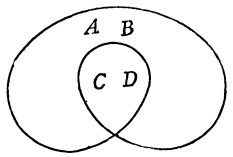
\includegraphics{scroll.png}
  \caption{Peirce's scroll}
  \labfig{scroll}
\end{marginfigure}

\reffig{scroll} shows Peirce's drawing of the scroll as it appears in
\cite[Fig.~5]{peirce_prolegomena_1906}. He defines its intended meaning like so
\cite[p.~534--535]{peirce_prolegomena_1906}:

\begin{quote}
  I shall call the outer boundary the Wall; and the inner, the Fence. In the
outer I scribed the Antecedent, in the inner the Consequent, of a Conditional
Proposition de inesse. [...][Thus the meaning of \reffig{scroll} is] that if
both A and B are true, then both C and D are true. [...] a Conditional de inesse
(unlike other conditionals) only asserts that either the antecedent is false or
the consequent is true. 
\end{quote}

This shows the classical view of Peirce on EG, who interprets the scroll as
signifying the \textit{conditional de inesse} --- also called nowadays
\emph{material implication}, and defined here in its disjunctive form, expressed
symbolically by $A \limp B \defeq \neg A \lor B$. This is no coincidence that
Peirce based his most fundamental icon on implication: according to Lewis
\sidecite[][p.~79]{Lewis1920-LEWASO-4}, he was the one who introduced the
``illative relation'' of implication into symbolic logic in the first place, by
giving it a distinguished symbol, and studying extensively the algebraic laws
that govern it (including Peirce's law).

\paragraph{Blank Antecedant}

\begin{marginfigure}
  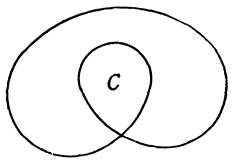
\includegraphics{empty-antecedant.png}
  \caption{Peirce's scroll with a blank antecedant}
  \labfig{empty-antecedant}
\end{marginfigure}

A first principle that Peirce derives from the scroll is the following
\cite[p.~534]{peirce_prolegomena_1906}:

\begin{quote}
  [...] any insertion [is] permitted in the outer close, and any omission from
the inner close. By applying the former clause of this rule to
[\reffig{empty-antecedant}], we see that this scroll with the outer close void,
justifies the assertion that if no matter what be true, C is in any case true;
so that the two walls of the scroll, when nothing is between them, fall
together, collapse, disappear, and leave only the contents of the inner close
standing, asserted, in the open field.
\end{quote}

This first form of ``collapsing of walls'' is called the \emph{Rule of Blank
Antecedant} in \cite{minghui_graphical_2019}, and corresponds symbolically to
the equivalence $\top \limp A \semequiv A$. The reader might be tempted to see
the ``former clause'' that permits any insertion in the outer close as a special
case of the Insertion principle of \sys{Alpha} (\refsec{alpha}). However, we
stress again that Peirce first identified this clause as a feature of the
scroll, seen as the diagrammatic embodiment of the ``general form of argument''
mentioned in a previous excerpt. The principle of Insertion only followed as a
subsequent generalization, stemming from the analysis of the scroll into two
nested cuts \cite[p.~535]{peirce_prolegomena_1906}:

\begin{quote}
  [...] and you will further see that a scroll is really nothing but one oval
within another.
\end{quote}

\begin{marginfigure}
  $$
  \!\!\!\!\stkfig{1}{scroll-empty-antecedant}
  \!\!\!\!\xinvstep{\rsf{BA}}~~~~
  G
  $$
  \caption{The rule of Blank Antecedant}
  \labfig{rule-empty-antecedant}
\end{marginfigure}

To emphasize this point, we will from now on depict scrolls as two nested cuts
joined at a single point highlighted in orange, as illustrated in
\reffig{rule-empty-antecedant}.

\begin{remark}
  It is interesting to note that the rule of Blank Antecedant is not seen as
  primitive by Peirce, but as a consequence of a \emph{dynamic potential} of the
  scroll: namely, the ability to insert anything in the outer close, at will.
  This is another manifestation of Peirce's concern for the question of
  \emph{illative atomicity}, and is to be related to the elimination of the
  Double-cut rule discussed in \refsec{atomicity}.
\end{remark}

\paragraph{Currying}

\begin{marginfigure}[-10em]
  ~~~\stkfig{0.8}{scroll-curried}
  \caption{Currying as scroll nesting}
  \labfig{scroll-curried}
\end{marginfigure}

\begin{marginfigure}[0em]
  \setlength{\fboxsep}{2pt}
\setlength{\arraycolsep}{0pt}
\newcommand{\vsp}{\vspace{-0.5em}}
\newcommand{\stkf}{\tikzfig{0.9}{0.5}}
$$
\begin{array}{r@{\quad}c@{\vsp}}
                                  &\stkf{eg-currying-3} \\
       \xstep{\kl{BA}} &\stkf{eg-uncurrying-1} \\
       \xstep{\kl{Ins}} &\stkf{eg-uncurrying-2} \\
       \xstep{\kl{Deit}} &\stkf{eg-currying-0}
\end{array}
$$
  \caption{Intuitionistic proof of currying}
  \labfig{eg-currying}
\end{marginfigure}

\begin{marginfigure}[27em]
  \setlength{\fboxsep}{2pt}
\setlength{\arraycolsep}{0pt}
\newcommand{\vsp}{\vspace{-0.5em}}
\newcommand{\stkf}{\tikzfig{0.9}{0.5}}
$$
\begin{array}{r@{\quad}c@{\vsp}}
                                  &\stkf{eg-currying-0} \\
       \xstep{\mathsf{Ins}} &\stkf{eg-currying-1} \\
       \xstep{\mathsf{Deit}} &\stkf{eg-currying-2} \\
       \xstep{\mathsf{BA}} &\stkf{eg-currying-3}
\end{array}
$$

  \caption{Intuitionistic proof of uncurrying}
  \labfig{eg-uncurrying}
\end{marginfigure}

Peirce was aware of the phenomenon of \emph{currying}, expressed symbolically by
the equivalence $A \limp B \limp C \semequiv A \land B \limp C$, as witnessed by
the following passage \cite[p.~535]{peirce_prolegomena_1906}:
\begin{quote}
Now, Reader, if you will just take pencil and paper and scribe the scroll
expressing that if $A$ be true, then it is true that if $B$ be true $C$ and $D$
are true [\reffig{scroll-curried}], and compare this with [\reffig{scroll}],
which amounts to the same thing in meaning, you will see that scroll walls with
a void between them collapse even when they belong to different scrolls.
\end{quote}
It is remarkable that he comes to this conclusion by a topological argument,
noting that this second form of ``collapsing of walls'', now involving two
different scrolls, follows from the scroll beeing composed of two nested cuts.
If we reject this interpretation by requiring that the Fence (the inner oval)
stays glued to the Wall (the outer oval), then one cannot derive currying
through the rule of double-cut, precisely because the system only permits to
collapse a Wall and a Fence continuously joined in the same scroll, by the
weaker rule of Blank Antecedant. Fear not however, as one can still derive the
currying and uncurrying laws in this intuitionistic setting, but through the
additional use of the insertion and deiteration rules, as depicted in
\reffig{eg-currying} and \reffig{eg-uncurrying}. Yet we find that Peirce's insight
on the topological explanation of currying in the classical setting remains
noteworthy.

\begin{remark}
Note that in \reffig{eg-currying} and \reffig{eg-uncurrying}, we give
\emph{direct} proofs that rewrite the premiss of the argument into its
conclusion, rather than \emph{goal-directed} proofs (\refdef{eg-proof}) that
rewrite a goal into the empty $\SA$, as we usually did in \refch{eg}. Direct
proofs are closer to Peirce's usage of the illative transformations --- and thus
to what can be found in most of the literature on EG, and have the advantage of
being more economical in space by leaving the goal implicit. One can easily go
from a direct proof to a goal-directed one as shown by the \emph{deduction
theorem} of Sowa \cite[Section 6]{sowa_peirces_2011}, which also applies
in the intuitionistic setting by substituting the rule of Double-cut with the
rule of Blank Antecedant.
\end{remark}

\paragraph{The $n$-ary scroll}

In \cite{oostra_graficos_2010}, A. Oostra proposes to take the above remark
seriously, by reifying the scroll as a primitive icon of EG (``\emph{rizo}'' in
Spanish), that exists alongside the cut (``\emph{corte}''), and is distinguished
from it. In fact he goes further than this, and proposes to generalize both the
cut and the scroll into an $n$-ary construction called the \emph{curl}
(``\emph{bucle}''), where $n$ is the number of inner closes, called \emph{loops}
(``\emph{lazos}''). \reffig{five-loops} shows an example of curl with five
loops. In \cite{minghui_graphical_2019}, the curl is simply called \emph{$n$-ary
scroll}, and is analyzed into the outer area (that enclosed by the Wall) called
the \emph{outloop}, and the inner areas (those enclosed by the $n$ Fences, i.e.
the loops of Oostra) called the \emph{inloops}. Then cuts and scrolls are indeed
special cases of $n$-ary scrolls, respectively with $n = 0$ and $n = 1$.

\begin{marginfigure}
  \stkfig{1}{five-loops}
  \caption{A curl with five loops}
  \labfig{five-loops}
\end{marginfigure}

Like the unary scroll, the $n$-ary scroll is to be read as an implication whose
antecedant is the content of the outloop, and consequent the content of the
inloops. The generalization then consists in taking the \emph{disjunction} of
the contents of all inloops: this reflects nicely the etymological meaning of
the word ``disjunction'', since the inloops enclose \emph{disjoint} areas of the
outloop to which they are attached. Then the $5$-ary scroll of
\reffig{five-loops} is read as the formula $a \limp b \lor c \lor d \lor e \lor
f$; and the $0$-ary scroll obtained by removing all inloops from the latter as
$a \limp \bot$, since a $0$-ary disjunction is naturally evaluated to its
neutral element $\bot$. This coincides with the intuitionistic reading of
negation $\neg A \defeq A \limp \bot$, and is thus consistent with the
interpretation of cuts as negations.

\paragraph{Continuity}

\begin{marginfigure}
  $$
\begin{array}{c}
  \begin{array}{cc}
    \stkfig{1}{scroll-disj} & A \lor B \\
    \stkfig{1}{scroll-imp} & A \limp B \\[1em]
    \multicolumn{2}{c}{\not=} \\
    \stkfig{1}{eg-disj} & \neg (\neg A \land \neg B) \\
    \stkfig{1}{eg-imp} & \neg (A \land \neg B)
  \end{array}
\end{array}
$$
  \caption{Continuity, disjunction and implication in IEG}
  \labfig{eg-disj-imp}
\end{marginfigure}

With this interpretation of the $n$-ary scroll, the \sys{Alpha} encodings of
disjunction and implication as nested cuts are no longer valid, because they are
not intuitionistically equivalent to the associated binary and unary scrolls.
This is illustrated in \reffig{eg-disj-imp}, where the closeness in meaning is
reflected iconically (but not symbolically) in the fact that the graphs only
differ in the \emph{continuity} (or lack thereof) between inloops and their
outloop. Indeed, contrary to nested cuts, any $n$-ary scroll can be drawn by a
\emph{continuous} movement of the pen, producing a self-intersecting curve as
described by Peirce in \cite{peirce_prolegomena_1906}. This might be related to
other manifestations of the notion of continuity in the semantics of
intuitionistic logic, such as the well-known Stone-Tarski interpretation of
formulas as topological spaces \cite{stone_topological_1938}, and the
interpretation of proofs as continuous maps in the \emph{denotational semantics}
of Dana Scott \sidecite{10.5555/218742.218744}. Before the advent of Oostra's
IEG, Zalamea gave a detailed analysis of Peirce's philosophy of
the \emph{continuum}, how it relates to modern developments in mathematics, and
how it is embodied in existential graphs \cite{zalamea_peirces_2003}. Actually
according to Oostra \sidecite[][p.~162]{oostra_advances_2022}, ``the
possibility of developing intuitionistic existential graphs was first suggested
by Zalamea in the 1990s \cite{zalamea_ieg_1}\cite{zalamea_ieg_2}''.

\paragraph{Coherent formulas}

\begin{marginfigure}
  $$
  \!\!\!\!
  \!\!\!\!
  \!\!\!\!
  \begin{array}{c}
    \tikzfig{0.85}{0.85}{curl-geom} \vspace{1.5em}\\
    \forall \mathbf{x}. \left(\bigwedge G \limp \bigvee_{j = 1}^{n}\exists \mathbf{x_j}. \bigwedge H_j\right)
  \end{array}
  $$
  \caption{Formula interpretation of the $n$-ary scroll}
  \labfig{curl-geom}
\end{marginfigure}

More generally, a $n$-ary scroll with atoms $G = a_1, \ldots, a_m$ in its outloop and
$\Delta = \begin{pmatrix}
  a_{1,1} & \ldots & a_{1,p_1} \\
  \vdots & \ddots & \vdots \\
  a_{n,1} & \ldots & a_{1,p_n}
\end{pmatrix}$
in its inloops, where each row $H_j$ in $\Delta$ encodes an inloop, can be
interpreted as the formula
$$\bigwedge_{i = 1}^{m}{a_i} \limp \bigvee_{j = 1}^{n}\bigwedge_{k = 1}^{p_n}{a_{j,k}}$$
If one adds \emph{binders} to the mix (see \refsec{gardens}) by having $\gamma =
\garden{\mathbf{x}}{G}$ as outloop, and
$\Xi = \begin{pmatrix}
  \mathbf{x_1} \\
  \vdots \\
  \mathbf{x_n}
\end{pmatrix} \cdot \Delta$ as inloops, then the interpretation is extended into
the formula
$$\forall \mathbf{x}. \left(\bigwedge_{i = 1}^{m}{a_i} \limp \bigvee_{j = 1}^{n}\exists \mathbf{x_j}. \bigwedge_{k = 1}^{p_n}{a_{j,k}}\right)$$
as depicted in \reffig{curl-geom}. Typically, the particular case where $\gamma
= \garden{x}{\emptyset}$ and $\Xi = (\emptyset) \cdot (p(x))$ encodes the graph
$$\stkfig{1}{scroll-forall}$$
expressing the universal quantification $\forall x. p(x)$, and the case where
$\gamma = \garden{\emptyset}{\emptyset}$ and $\Xi = (x) \cdot (p(x))$ the graph
$$\stkfig{1}{scroll-exists}$$
expressing the existential quantification $\exists x. p(x)$. The interpretation
is invariant under polarity, meaning that for instance the graphs
$$\stkfig{1}{scroll-neg-forall} \text{   and   } \stkfig{1}{scroll-neg-exists}$$
obtained by enclosing the previous graphs in a cut are interpreted with the same
quantifiers, as the formulas $\neg \forall x. p(x)$ and $\neg \exists x. p(x)$.
In \sys{Beta}, we would have exploited the classical equivalences $\neg \forall
x. A \semequiv \exists x. \neg A$ and $\neg \exists x. A \semequiv \forall x.
\neg A$ (justified by the double-cut principle) in order to interpret them as
$\exists x. \neg p(x)$ and $\forall x. \neg p(x)$, emphasizing the idea that
positive and negative binders encode respectively $\exists$ and $\forall$. But
this is not possible anymore with the intuitionistic interpretation of $n$-ary
scrolls, where the $\exists/\forall$ duality is replaced by the inloop/outloop
distinction. In fact, we are tempted to further qualify this distinction of
\emph{adjunction}, following a classical result of Lawvere in the context of
categorical logic \sidecite{lawvere_quantifiers_sheaves}.

Lawvere is also known for some contributions to the study of \emph{geometric
logic} \sidecite{lawvere_geometric}, a subset of the formulas of FOL first
discovered by Skolem \sidecite{skolem_geometric} that is capable of expressing
many mathematical theories, and has close connections to \emph{topos theory}.
Quite remarkably, the interpretation of $n$-ary scrolls coincides exactly with
the class of \emph{coherent formulas}, which are the formulas of geometric logic
where infinitary disjunctions are restricted to finitary ones. There is a
difference however: the full syntax of IEG allows for arbitrary \emph{nestings}
of $n$-ary scrolls inside eachother, i.e. the multisets $G$ and $H_j$ in
\reffig{curl-geom} can contain $n$-ary scrolls in addition to atoms; while
coherent formulas are restricted to atoms.

Coherent formulas have some nice proof-theoretical properties, which might also
apply to IEG to some extent. We only mention two important ones:
\begin{description}
  \item[Completeness] Every first-order theory has a coherent conservative
  extension, making coherent formulas (and thus non-nested $n$-ary scrolls) in
  principle as expressive as arbitrary first-order formulas
  \sidecite{negri_geometric}.
  
  \item[Automation] Coherent formulas benefit from faster proof-search
  procedures compared to arbitrary formulas, making automation more tractable
  computationally. They also allow the direct encoding of many reasoning
  problems, thanks to their use of the full set of connectives and quantifiers
  of FOL; and avoiding complex encodings (as can be found e.g. in SMT solvers)
  is crucial in \emph{interactive} theorem proving, where the user and the
  computer manipulate the same formulas in goals
  \sidecite{bezem_automating_2005}. This has been exploited already in some
  domain-specific theorem provers, like the Larus prover that automatically
  generates illustrated proofs in geometry\sidenote{Incidentally, projective
  geometry was one of the motivating applications that led Skolem to identify
  the class of coherent formulas \cite{bezem_automating_2005}.}
  \sidecite{narboux_larus}.
  
  \begin{remark}
  Thus with IEG, one becomes able to reason \emph{geometrically} on geometric
  formulas that speak about geometry: another beautiful incarnation of the
  reflexivity at work in Peirce's iconic logic.
  \end{remark}
\end{description}

\section{Flowers}\labsec{Flowers}

\paragraph{Blooming}

As we have seen, the ($n$-ary) scroll is a powerful icon, because it captures
the distinction between classical and intuitionistic logic as being a matter of
\emph{continuity} between the space of inputs/hypotheses (outloop) and the
spaces of outputs/conclusions (inloops), reflecting an intuition discovered much
later in the denotational semantics of the $\lambda$-calculus. However as a
diagrammatic component to be operated upon through direct manipulation, it has
one notable flaw, also shared with the classical cut-based syntax: it quickly
induces heavy nestings of curves in the plane, making even a simple graph like
that of \reffig{scroll-curried} hard to read for an untrained eye.

\begin{marginfigure}
  $$
  \tikzfig{1}{0.4}{scroll-inside-out}
  $$
  \caption{Turning a $5$-ary scroll inside-out}
  \labfig{scroll-inside-out}
\end{marginfigure}

Before devising an alternative syntax, one should ask: what are the essential
features of the scroll that we want to preserve? Following the previous
observations, we identified two of them:
\begin{itemize}
  \item[\textbf{Continuity}] the scroll is a self-intersecting continuous curve,
  which can be drawn in one stroke of the pen;
  \item[\textbf{Polarity}] this curve delineates two kinds of areas: inloops that have
  the same polarity as the area on which the scroll is scribed, and the outloop
  which has the opposite polarity.
\end{itemize}

Fortunately, these two properties are preserved when turning inloops
\emph{inside-out}, as illustrated in \reffig{scroll-inside-out}. This might be
because the very process of turning inside-out can be seen as a continuous
movement in three-dimensional space, where the inloops are rotated around their
intersection points with the outloop. In this way, we have effectively divided
the amount of curve-nesting in scrolls by two. And as an added bonus, the new
icon is reminiscent of a \emph{flower}, as if it had bloomed from its curled
bud; or as if the pistol from \reffig{five-loops} had transformed into a
\emph{pistil}, and its bullet chambers into \emph{petals}\sidenote{As the saying
goes: make love, not war.}.

\begin{marginfigure}
  $$
  \!\!\!\!
  \!\!\!\!
  \!\!\!\!
  \!\!\!\!
  \stkfig{0.65}{flowers}
  $$
  \vspace{-3em}
  \caption{Nested flowers}
  \labfig{flowers}
\end{marginfigure}

From that point onwards, we decided to fully embrace the flower metaphor: first
in our drawing style as witnessed in \reffig{flowers}, but also in our syntactic
terminology, to be introduced in the next pages. Negative outloops are now drawn
as \emph{yellow} pistils for a more colorful experience, and inloops as
transparent petals, i.e. of the same color as the area on which they are
scribed. We also drop the requirement that petals should intersect their pistil
at a single point, for purely aesthetic reasons.

\paragraph{Multisets}

As we did for classical EG in \refsec{multisets} and \refsec{gardens}, we are
now going to distill the syntactic essence of flowers into an inductive,
(multi)set-based data structure. This will allow for a more compact textual
notation, that is better suited to proof-theoretical study.

In \refsec{beta}, we explained how the graphs of \sys{Beta} allow to represent
purely relational statements, without function symbols. Since functions are just
deterministic relations, one can in principle formalize any first-order theory
in this syntax\sidenote{Conversely, every relation can be faithfully encoded as
its characteristic function, which is the basis for the formalization of
mathematics in \emph{type theories}.}. However it is much more convenient to
have a dedicated syntax for functions, and we will thus introduce them as is
usually done in predicate calculus.

\begin{definition}[First-order signature]
  A \emph{first-order signature} is a triplet $\mathcal{\Sigma} = (
  \fsymbs, \psymbs, \arity )$, where $\fsymbs$ and $\psymbs$ are
  respectively the countable sets of \emph{function} and \emph{predicate}
  symbols of $\Sigma$, and $\arity : \fsymbs \cup \psymbs \to \nats$ gives an
  \emph{arity} to each symbol.
\end{definition}

In the following, we assume given a denumerable set of variables $\vars$
and a first-order signature $\Sigma$.

\begin{definition}[Terms]
  The set of terms $\terms$ is defined inductively as follows:
  \begin{itemize}
    \item{\textbf{(Variable)}} If $x \in \vars$ then $x \in \terms$;
    \item{\textbf{(Application)}} If $f \in \fsymbs$ and $\tvec{t}
    \in \terms^{\arity(f)}$, then $f(\tvec{t}) \in \terms$.
  \end{itemize}
\end{definition}

\begin{definition}[Flowers]\labdef{flowers}
  The sets of \emph{flowers} $\flowers$ and \emph{gardens} $\gardens$ are
  defined mutually inductively as follows:
  \begin{itemize}
    \item{\textbf{(Atom)}} If $p \in \psymbs$ and $\tvec{t} \in
    \terms^{\arity(p)}$, then $p(\tvec{t}) \in \flowers$;
    \item{\textbf{(Garden)}} If $\mathbf{x} \subset \vars$ is a finite set and $\Phi
    \subset \flowers$ a finite multiset, then $\garden{\mathbf{x}}{\Phi} \in
    \gardens$;
    \item{\textbf{(Flower)}} If $\gamma \in \gardens$ and $\Delta \subset \gardens$
    is a finite multiset, then $\flower{\gamma}{\Delta} \in \flowers$.
  \end{itemize}
\end{definition}

Any finite set $\mathbf{x} \subset \vars$ of variables is called a
\emph{sprinkler}, finite multiset $\Phi \subset \flowers$ of flowers a
\emph{bouquet}, and finite multiset $\Gamma \subset \gardens$ of gardens a
\emph{corolla}. We will often write gardens as $\garden{x_1, \ldots,
x_n}{\phi_1, \ldots, \phi_m}$, where the $x_i$ are called \emph{binders}; and
non-atomic flowers as $\flower{\gamma}{\delta_1 \sep \ldots \sep \delta_n}$,
where $\gamma$ is the \emph{pistil}, and the $\delta_i$ are called
\emph{petals}. We write $\fset{i}{n}{E_i}$ to denote a finite (multi)set of size
$n$ with elements $E_i$ indexed by $1 \leq i \leq n$. We also omit writing the
empty (multi)set, accounting for it with blank space as is done in sequent
notation\sidenote{Seen as sequents, the nesting of flowers might be related to
the nesting of judgments in the category of judgments used in the definition of
some recent categorical semantics of type theory \cite{huang2023synthetic}.} or
in EG; in particular, $\garden{{}}{{}}$ stands for the empty garden
$\garden{\emptyset}{\emptyset}$, $\flower{\gamma}{{}}$ for the flower with no
petals $\flower{\gamma}{\emptyset}$, and $\flower{\gamma}{\garden{{}}{{}}}$ for
the flower with one empty petal.

Note that the order of precedence of operators is
$\mathop{,} < \garden{{}}{{}} < \mathop{;} < \mathop{\flower{}{}}$
so that for instance, the string
$$\flower{\garden{x_1, x_2}{\phi_1, \phi_2}}{\garden{y_1}{\psi, (\flower{\gamma}{\Delta})} \sep \garden{y_2}{\Phi}}$$
is parsed as the flower
% $$\left(\flower{\left(\garden{\{x_1, x_2\}}{\{\phi_1,
% \phi_2\}}\right)}{\{\left(\garden{\{y_1\}}{\{\psi,
% \left(\flower{\gamma}{\Delta}\right)\}}\right) \sep
% \left(\garden{\{y_2\}}{\Phi}\right)\}}\right)$$ where constructed finite
% (multi)sets are delimited with $\{\}$, and constructed flowers/gardens are
% delimited with $()$.
\vspace{-6em}
$$\stkfig{1}{parsed-flower}$$
\vspace{-6em}

Also to improve readability, we will most of the time omit the garden dot
`$\cdot$' when the sprinkler is empty, writing $\Phi$ instead of
$\garden{{}}{\Phi}$.

\begin{remark}
  In some places the choice of letter for meta-variables will be important to
  disambiguate the kind of syntactic object we denote. \reftab{letters}
  summarizes our chosen notational conventions in this respect.
\end{remark}

\begin{marginfigure}
  \centering
  \begin{tabular}{|c|c|}
    \hline
    \bfseries Kind & \bfseries Letters \\
    \hline
    Variables ($\vars$) & $x, y, z$ \\
    Terms ($\terms$) & $t, u, v$ \\
    Flowers ($\flowers$) & $\phi, \psi, \xi$ \\
    Gardens ($\gardens$) & $\gamma, \delta$ \\
    Sprinklers & $\mathbf{x}, \mathbf{y}, \mathbf{z}$ \\
    Term vectors & $\tvec{t}, \tvec{u}, \tvec{v}$ \\
    Substitutions & $\sigma, \tau$ \\
    Bouquets & $\Phi, \Psi, \Xi$ \\
    Corollas & $\Gamma, \Delta$ \\
    Contexts & $\Phi\hole, \Psi\hole, \Xi\hole$ \\
    Theories & $\mathcall{T}, \mathcall{U}$ \\
    \hline
  \end{tabular}
  \caption{Notational conventions for meta-variables}
  \labtab{letters}
\end{marginfigure}

We now proceed with routine definitions for handling variables and substitutions
of terms in flowers.

\begin{definition}[Free variables]\labdef{fv}
  The sets of \emph{free variables} $\fv(-)$ of a term, flower or garden are
  defined mutually recursively as follows:
  \begin{align*}
    \fv(x) &= \{x\} \\
    \fv(f(\tvec{t})) &= \bigcup_{t \in \tvec{t}}{\fv(t)} \\
    \fv(p(\tvec{t})) &= \bigcup_{t \in \tvec{t}}{\fv(t)} \\
    \fv(\garden{\mathbf{x}}{\Phi}) &= \bigcup_{\phi \in \Phi}{\fv(\phi)} \setminus \mathbf{x} \\
    \fv(\flower{\garden{\mathbf{x}}{\Phi}}{\Delta}) &= \fv(\garden{\mathbf{x}}{\Phi}) \cup \bigcup_{\garden{\mathbf{y}}{\Psi} \in \Delta}{\fv(\garden{\mathbf{x}, \mathbf{y}}{\Psi})}
  \end{align*}
  We say that a term, flower or garden is \emph{closed} when its set of free
  variables is empty. The sets of closed terms, flowers and gardens are denoted
  respectively by $\closed{\terms}$, $\closed{\flowers}$ and $\closed{\gardens}$.
\end{definition}

\begin{remark}\labremark{flower-scope}
Note that the scope of a binder located in a pistil extends both to the pistil
\emph{and} to all its attached petals, whereas for a binder located in a petal
it is limited to said petal. This is reflected in the above definition of free
variables for (non-atomic) flowers, and is visually explained by the nesting of
curves in an $n$-ary scroll.
\end{remark}

\begin{definition}[Bound variables]
  % The set of \emph{bound variables} $\bv(\Phi\hole)$ of a context $\Phi\hole$ is defined
  % inductively as follows:
  % \begin{align*}
  %   \bv(\Psi, \hole) &= \emptyset \\
  %   \bv(\Psi, (\flower{\garden{\mathbf{x}}{X}}{\Delta})) &= \mathbf{x} \cup \bv(X) \\
  %   \bv(\Psi, (\flower{\garden{\mathbf{x}}{\Phi}}{\garden{\mathbf{y}}{X} \sep \Delta})) &= \mathbf{x} \cup \mathbf{y} \cup \bv(X)
  % \end{align*}
  The set of bound variables $\bv(\phi)$ (resp. $\bv(\gamma)$) of a flower
  $\phi$ (resp. garden $\gamma$) is defined mutually recursively as follows:
  \begin{align*}
    \bv(p(\tvec{t})) &= \emptyset \\
    \bv(\garden{\mathbf{x}}{\Phi}) &= \mathbf{x} \cup \bigcup_{\phi \in \Phi}{\bv(\phi)} \\
    \bv(\flower{\gamma}{\Delta}) &= \bv(\gamma) \cup \bigcup_{\delta \in \Delta}{\bv(\delta)}
  \end{align*}
\end{definition}

To avoid reasoning about $\alpha$-equivalence, we adopt in this work the
so-called \emph{Barendregt convention} that all variable binders are distinct,
both among themselves and from eventual free variables. Formally, we assume that
for any flower $\phi$, the two following conditions hold:
\begin{enumerate}
  \item computing $\bv(\phi)$ as a multiset gives the same result as computing
  it as a set;
  \item $\bv(\phi) \cap \fv(\phi) = \emptyset$.
\end{enumerate} 
% To preserve this convention, in this paper we will only consider
% \emph{non-circular} substitutions $\sigma$ where $x \not\in \fv(\sigma(x))$ for
% all $x \in \dom(\sigma)$.

To define substitutions, we introduce a general notion of \emph{function
update}, which will be useful for the semantic evaluation of flowers in
\refsec{Semantics}.

\begin{definition}[Function update]
  Let $A, B$ be two sets, $f, g : A \to B$ two functions and $R \subseteq A$
  some subset of their domain. The \emph{update} of $f$ on $R$ with $g$ is the
  function defined by:
  $$
  (\update{f}{R}{g})(x) =
  \begin{cases}
    g(x) &\text{if $x \in R$} \\
    f(x) &\text{otherwise}
  \end{cases}
  $$
  $\update{-}{-}{-}$ is obviously associative, that is
  $\update{f}{R}{(\update{g}{S}{h})} = \update{(\update{f}{R}{g})}{S}{h}$. Also
  if $f$ or $g$ is the identity function $\idsubst$ we omit writing it, i.e.
  $\update{f}{R}{{}} = \update{f}{R}{\idsubst}$ and $\update{{}}{R}{g} =
  \update{\idsubst}{R}{g}$.
\end{definition}

\begin{definition}[Substitution]
  A \emph{substitution} is a function $\sigma : \vars \to \terms$ with a finite
  \emph{support} $\dom(\sigma) = \compr{x}{\sigma(x) \not= x}$. By abuse of
  notation, we will write $\sigma : \mathbf{x} \to \terms$ to denote a
  substitution $\sigma$ whose support is $\mathbf{x}$. The domain of
  substitutions is extended to terms, flowers and gardens mutually recursively
  as follows:
  \begin{align*}
    \sigma(f(x_1, \ldots, x_n)) &= f(\sigma(x_1), \ldots, \sigma(x_n)) \\
    \sigma(p(\tvec{t})) &= p(\sigma(\tvec{t})) \\
    \sigma(\garden{\mathbf{x}}{\Phi}) &=
      \garden{\mathbf{x}}{\restr{\sigma}{\mathbf{x}}(\Phi)} \\
    \sigma(\flower{\garden{\mathbf{x}}{\Phi}}{\Delta}) &=
      \flower{\sigma(\garden{\mathbf{x}}{\Phi})}{\restr{\sigma}{\mathbf{x}}(\Delta)}
  \end{align*}
\end{definition}

\section{Calculus}\labsec{Calculus}

\paragraph{Contexts}

Equipped with an inductive syntax, we can now express formally the inference
rules of our flower calculus, just as we did for \sys{Alpha}
(\refsec{multisets}) and \sys{Beta} (\refsec{gardens}). There, graphs and their
contexts were defined as multisets of nodes, which have now turned into bouquets
of flowers:

\begin{definition}[Bouquet context]
  A \emph{bouquet context} $\Phi\hole$ is a bouquet which contains exactly one
  occurrence of the special flower $\hole$ called the \emph{hole}. The hole can
  always be \emph{filled} (substituted) with any other bouquet $\Psi$ or context
  $\Xi\hole$, producing a new bouquet $\cfill{\Phi}{\Psi}$ or context
  $\cfill{\Phi}{\Xi\hole}$. In particular, filling with the empty bouquet will
  yield a bouquet $\cfill{\Phi}{\phantom{\Phi}}$, which is just $\Phi\hole$ with
  its hole removed.
\end{definition}

\begin{definition}[Parity]
  The \emph{parity} $\parity{\Phi\hole}$ of a context $\Phi\hole$ is defined
  mutually recursively by:
  \begin{align*}
    \parity{\Psi, \hole} &= 0 \\
    \parity{\Psi, (\flower{\garden{\mathbf{x}}{\Phi\hole}}{\Delta})} &= \parity{\Phi\hole} + 1 \\
    \parity{\Psi, (\flower{\gamma}{\garden{\mathbf{x}}{\Phi\hole} \sep \Delta})} &= \parity{\Phi\hole}
  \end{align*}
\end{definition}

\begin{definition}[Polarity]
  We say that a context $\Phi\hole$ is \emph{positive} if $\parity{\Phi\hole}$ is even, and
  \emph{negative} otherwise. We denote positive and negative contexts
  respectively by $\Phi^+\hole$ and $\Phi^-\hole$.
\end{definition}

\paragraph{Pollination}

In order to formulate the equivalent of the (de)iteration rules of EG for
flowers, we introduce a \emph{pollination} relation that captures the
availability of a flower in a given context, akin to the \emph{justification}
relation of \refsec{atomicity}:

\begin{definition}[Pollination]\labdef{pollination}
  We say that a flower $\phi$ can be \emph{pollinated} in a context $\Phi\hole$,
  written $\chyp{\phi}{\Phi\hole}$, when there exist a bouquet $\Psi$ with $\phi
  \in \Psi$ and contexts $\Xi\hole$ and $\Xi_0\hole$ such that either:
  \begin{itemize}
    \item (\textbf{Cross-pollination})~ $\Phi\hole = \cfill{\Xi}{\Psi,
    \Xi_0\hole}$;
    \item (\textbf{Self-pollination})~ $\Phi\hole =
    \cfill{\Xi}{\flower{\garden{\mathbf{x}}{\Psi}}{\garden{\mathbf{y}}{\Xi_0\hole}
    \sep \Delta}}$ for some $\mathbf{x}, \mathbf{y}, \Delta$.
  \end{itemize}
  A bouquet $\Psi$ can be pollinated in $\Phi\hole$, written
  $\chyp{\Psi}{\Phi\hole}$, if $\chyp{\psi}{\Phi\hole}$ for all $\psi \in \Psi$.
\end{definition}

\begin{marginfigure}
  $$
  \!\!\!\!
  \!\!\!\!
  \!\!\!\!
  \begin{array}{c}
    \tikzfig{1}{0.5}{cross-pollination} \vspace{-2em} \\
    \text{\textit{Cross-pollination}} \vspace{-1em} \\
    \tikzfig{1}{0.5}{self-pollination} \vspace{-2em} \\
    \text{\textit{Self-pollination}}
  \end{array}
  $$
  \caption{Pollination in flowers}
  \labfig{pollination}
\end{marginfigure}

We now employ the metaphor of \emph{pollination} to speak about (de)iteration in
flowers. This is illustrated in \reffig{pollination}, where the blue dot marks
the location of the justifying/pollinating occurrence of $\phi$, and the red
dots all the areas that it (locally) justifies/pollinates, and thus where $\phi$
can be (de)iterated\sidenote{\reffig{pollination} summarizes visually the flow
of information in flowers, just like \reffig{eg-local-justification} summarized
the flow of information in EG, and \reffig{bubbles-porosity} in bubbles. From a
UI point of view, all these figures can be understood as kind of
``cheatsheets'', that indicate with arrows the allowed drag-and-drop moves for
importing a statement (the source of the DnD) into a new context (the
destination of the DnD).}. We distinguish two cases of \emph{cross}-pollination
and \emph{self}-pollination, as botanists do when describing the reproduction of
flowers. This distinction does not exist in classical EG, because pistils and
petals are both identified as instances of cuts. If we were to replace binders
by LoI (lines of identity, see \refsec{beta}), then the pollination relation
would also prescribe in which areas LoI can be extended/iterated, providing an
explanation for the scope of binders (\refremark{flower-scope}).

\paragraph{Rules}

\begin{figure*}
  \begin{framed}
{\textsc{Nature} $\intro*\Nature$}
\vspace{1.5em}
\begin{mathpar}
  \R[\intro{poll{\da}}]
    {\cfill{\Xi}{\phantom{\Phi}}}
    {\cfill{\Xi}{\Phi}}
  \and
  \R[\intro{poll{\ua}}]
    {\cfill{\Xi}{\Phi}}
    {\cfill{\Xi}{\phantom{\Phi}}}
  \\
  \R[\intro{epis}]
    {\flower{\garden{{}}{{}}}{\garden{{}}{\Phi}}}
    {\Phi}
  \and
  \R[\intro{epet}]
    {}
    {\flower{\gamma}{\garden{{}}{{}} \sep \Delta}}
  \\
  \R[\intro{ipis}]
    {(\flower{\garden{\bx}{\sigma(\Phi)}}{\sigma(\Delta)}), (\flower{\garden{\bx, \by}{\Phi}}{\Delta})}
    {\flower{\garden{\bx, \by}{\Phi}}{\Delta}}
  \and
  \R[\intro{ipet}]
    {\flower{\gamma}{\garden{\bx}{\sigma(\Phi)} \sep \garden{\bx, \by}{\Phi} \sep \Delta}}
    {\flower{\gamma}{\garden{\bx, \by}{\Phi} \sep \Delta}}
  \\
  \R[\intro{srep}]
    {\flower{\garden{\bx}{\Phi}}{\garden{{}}{\fset{i}{n}{\flower{\gamma_i}{\Delta}}}}}
    {\flower{\garden{\bx}{\Phi, (\flower{\garden{{}}{{}}}{\fset{i}{n}{\gamma_i}})}}{\Delta}}
\end{mathpar}

\vspace{3em}

{\textsc{Culture} $\intro*\Culture$}
\vspace{1.5em}
\begin{mathpar}
  \R[\intro{grow}]
    {\cfill{\Xi^+}{\Phi}}
    {\cfill{\Xi^+}{\phantom{\Phi}}}
  \and
  \R[\intro{crop}]
    {\cfill{\Xi^-}{\phantom{\Phi}}}
    {\cfill{\Xi^-}{\Phi}}
  \\\\
  \R[\intro{pull}]
    {\cfill{\Xi^+}{\flower{\gamma}{\Delta}}}
    {\cfill{\Xi^+}{\flower{\gamma}{\Gamma \sep \Delta}}}
  \and
  \R[\intro{glue}]
    {\cfill{\Xi^-}{\flower{\gamma}{\Gamma \sep \Delta}}}
    {\cfill{\Xi^-}{\flower{\gamma}{\Delta}}}
  \\\\
  \R[\intro{apis}]
    {\cfill{\Xi^+}{\flower{\garden{\bx, \by}{\Phi}}{\Delta}}}
    {\cfill{\Xi^+}{\flower{\garden{\bx}{\sigma(\Phi)}}{\sigma(\Delta)}}}
  \and
  \R[\intro{apet}]
    {\cfill{\Xi^-}{\flower{\gamma}{\garden{\bx, \by}{\Phi} \sep \Delta}}}
    {\cfill{\Xi^-}{\flower{\gamma}{\garden{\bx}{\sigma(\Phi)} \sep \Delta}}}
\end{mathpar}

\vspace{3em}

In the rules \kl{poll{\da}} and \kl{poll{\ua}}, we assume that
$\chyp{\Phi}{\Xi\hole}$.

In the rules \kl{ipis}, \kl{apis} (resp. \kl{ipet}, \kl{apet}), we
assume some \kl{substitution} $\sigma : \by \to \terms$ that is
capture-avoiding in $\flower{\garden{{}}{\Phi}}{\Delta}$ (resp. $\Phi$).
\end{framed}
  \caption{Rules of the flower calculus}
  \labfig{flower-calculus}
\end{figure*}

\begin{figure*}
  \newcommand{\tkfig}[2]{\tikzfig{#1}{1}{#2}}
\newcommand{\st}[1]{\xstep{#1}}
\begin{framed}
{\textsc{Nature} $\Nature$}
\vspace{1.5em}
\begin{mathpar}
  \begin{array}{rcl}
    \tkfig{0.8}{srep-1} &
    \st{\rsf{srep}} &
    \!\!\!\!\!\!\!\!\tkfig{0.8}{srep-2}
  \end{array}
\end{mathpar}

% \vspace{3em}

% {\textsc{Culture} $\Culture$}
% \vspace{1.5em}
% \begin{mathpar}
% \end{mathpar}

% \vspace{3em}

% In the rules \rnmsf{poll{\da}} and \rnmsf{poll{\ua}}, we assume that
% $\chyp{\Phi}{\Xi\hole}$.

% In the rules \rnmsf{ipis}, \rnmsf{ipet}, \rnmsf{apis}, \rnmsf{apet}, we assume
% some substitution $\sigma : \mathbf{y} \to \terms$.
\end{framed}
  \caption{Graphical presentation of the flower calculus}
  \labfig{flower-calculus-graphical}
\end{figure*}

As has become standard in this thesis, we define the flower calculus as a
\emph{rewriting system} on bouquets, presented in \reffig{flower-calculus} as a
set of unary deep inference rules: when read \emph{top-down}, they correspond to
usual inferences from premiss to conclusion, and will be justified by the
soundness theorem of \refsec{Soundness}.
% This gives them a \emph{static}, \emph{a posteriori} meaning, since this is
% typically how you would check the validity of an established inference
% \emph{after the fact}.
But the more interesting direction, and the one around which the calculus has
been designed, is when you read the rules \emph{bottom-up}: then they are indeed
rewrite rules, telling you the different ways in which you can choose to
simplify a goal. This is how the \emph{graphical} version of the rules is
presented in \reffig{flower-calculus-graphical}.

Let us now describe the rules in more detail, starting with the fragment that is
a direct adaptation of the rules of \sys{Beta} (\reffig{beta}):

\begin{description}
  \item[Blank Antecedant (\rsf{epis})]
    It allows to enclose any bouquet in a petal attached to an
    \textsf{(e)}mpty \textsf{(pis)}til. This is one
    direction of the rule \rsf{BA} of (\reffig{rule-empty-antecedant}), which is
    a weaker, intuitionistic version of the classical rule \rsf{Dcut{\ua}} of
    \sys{Alpha} and \sys{Beta}. The other direction is actually unnecessary for
    completeness, which might be related to the co-admissibility of
    \rsf{Dcut{\da}} in \sys{Alpha} (Corollary \ref{cor:adm-ins}).

  \item[(De)iteration (\rsf{poll{\da}}, \rsf{poll{\ua}})]
    Renamed \emph{\textsf{(poll)}ination} rules, they correspond to the rules
    \rsf{Iter} and \rsf{Deit} of \sys{Alpha} and \sys{Beta}, but reformulated
    with the pollination relation (\refdef{pollination}).

  \item[Insertion/Deletion (\rsf{grow}, \rsf{crop}, \rsf{pull}, \rsf{glue})]
    They correspond to the rules \rsf{Ins} and \rsf{Del} of \sys{Alpha} and
    \sys{Beta}, but have doubled in number to account for the syntactic
    distinction between pistils and petals. More precisely, rules \rsf{grow} and
    \rsf{crop} allow to insert and delete entire flowers, while rules \rsf{pull}
    and \rsf{glue} deal with petals.
    
  \item[Unification (\rsf{ipis}, \rsf{ipet}, \rsf{apis}, \rsf{apet})]
    Rules \rsf{ipis} and \rsf{ipet} allow to \textsf{(i)}nstantiate a sprinkler
    located respectively in a \textsf{(pis)}til ($\forall$) and a
    \textsf{(pet)}al ($\exists$) with an arbitrary substitution, while rules
    \rsf{apis} and \rsf{apet} do the opposite operation of
    \textsf{(a)}bstracting a set of terms by introducing a sprinkler. They
    correspond respectively to a generalization of the rules \rsf{Unif{\ua}} and
    \rsf{Unif{\da}} of \sys{Beta}, where the variable substitution $\{z/y\}$
    becomes an arbitrary substitution $\sigma$. Once again, we have twice the
    amount of rules to account for the pistil/petal distinction, which is not
    surprising since in the LoI syntax of EG, they are special cases of
    Insertion/Deletion. Note that for the instantiation rules
    \rsf{ipis}/\rsf{ipet} to be invertible, we duplicate the whole flower/petal
    where the sprinkler occurs, mirroring what is done in multi-conclusion
    sequent calculi (see \reffig{multi-inst}).
\end{description}

The last two rules handle the behavior of disjunctive and absurd statements,
i.e. flowers with respectively $n \geq 2$ and $n = 0$ petals, and are closer to
sequent-style introduction/elimination rules:

\begin{description}
  \item[Disjunction Introduction (\rsf{epet})]
    It allows to erase any flower with an \textsf{(e)}mpty \textsf{(pet)}al.
    According to Oostra \cite[p.~109]{oostra_advances_2022}, Peirce already
    identified \rsf{epet} as a component of his decision procedure for \sys{Alpha}
    (it is simply called ``Operation 1'' in \cite{oostra_advances_2022}). This is
    no coincidence, since we precisely came up with this rule when trying to
    design a decision procedure for flowers.

  \item[Disjunction/Falsity Elimination (\rsf{srep})]
    It corresponds to a $n$-ary generalization of the left introduction rule for
    disjunction in sequent calculus, the $0$-ary case capturing falsity
    elimination (\textit{ex falso quodlibet}). The binary case is also used in
    the IEG system of \cite{minghui_graphical_2019}, together with its converse.
    The name \rsf{srep} is short for \textsf{(s)}elf-\textsf{(rep)}roduction,
    which is more clearly visualized in the graphical version of the rule in
    \reffig{flower-calculus-graphical}. Through the Curry-Howard correspondence,
    it can be related to the \emph{pattern-matching generator} found in modern
    editors of some functional programming languages, such as the Hazel
    structure editor \sidecite{yuan-live-2023}, and the Agda proof assistant.
\end{description}

\paragraph{Proofs}

Our notions of derivation and proof are essentially the same as the ones given
for EG in \refsec{multisets}, except that we distinguish from the outset between
two kinds of derivations, stemming from our partitioning of the rules into two
sets: the \emph{natural} rules denoted by $\Nature$, and the \emph{cultural}
rules denoted by $\Culture$. In particular, every natural rule in $\Nature$ is
both \emph{analytic} (i.e. every atom in the premiss already appears in the
conclusion) and \emph{invertible} (this will be shown in \refsec{Soundness});
and we will prove in \refsec{Completeness} that the entire cultural fragment
$\Culture$ is \emph{admissible}.

\begin{definition}[Derivation]
  Given a set of rules $\mathsf{R}$, we write $\Phi \step_{\mathsf{R}} \Psi$ to
  indicate a rewrite \emph{step} in $\mathsf{R}$, that is an instance of some $r
  \in \mathsf{R}$ with $\Psi$ as premiss and $\Phi$ as conclusion. We just write
  $\Phi \step \Psi$ to mean $\Phi \step_{\Nature\cup\Culture} \Psi$. A
  \emph{derivation} $\Phi \nsteps{n}_{\mathsf{R}} \Psi$ is a sequence of rewrite
  steps $\Phi_0 \step_{\mathsf{R}} \Phi_1 \ldots \step_{\mathsf{R}} \Phi_n$ with
  $\Phi_0 = \Phi$, $\Phi_n = \Psi$ and $n \geq 0$. Generally the length $n$ of
  the derivation does not matter, and we just write $\Phi \steps_R \Psi$.
  Finally, natural derivations are closed under arbitrary contexts: for every
  context $\Xi\hole$, $\Phi \step_\Nature \Psi$ implies $\cfill{\Xi}{\Phi}
  \step_\Nature \cfill{\Xi}{\Psi}$. We write $\Phi \lstep_{\Nature} \Psi$ to
  denote a \emph{local} natural step, i.e. a direct instance of a natural rule
  in the empty context.
\end{definition}

\begin{definition}[Proof]\labdef{flowers-proof}
  A \emph{proof} of a bouquet $\Phi$ is a derivation $\Phi \steps \emptyset$.
\end{definition}

In Peircean terms, the empty bouquet is the blank sheet of assertion, which as
we have seen in \refsec{alpha} can be interpreted as the icon of \emph{absolute
truth}. Then in our proof construction paradigm, proving a bouquet amounts to
erasing it completely from the sheet of assertion, thus reducing it to absolute
truth.

Now if we want to speak about \emph{relative} truth $\Psi \vdash \Phi$, i.e.
$\Phi$ is true under the assumption that $\Psi$ is, it turns out that the notion
of natural derivability $\Phi \steps_{\Nature} \Psi$ is too weak. Indeed as
already mentioned, the natural rules of the flower calculus are both
\emph{invertible} and \emph{complete} for provability. A consequence of
invertibility is that natural derivability is only able to relate logically
equivalent bouquets --- in fact not even all of them --- which prevents the
applicability of the \emph{deduction theorem} (\refthm{deduction}). That is, as
soon as $\flower{\Psi}{\Phi}$ is provable but the converse $\flower{\Phi}{\Psi}$
is not, it will necessarily follow that $\Phi \not\steps_{\Nature} \Psi$. This
problem does not arise if we consider full derivability $\Phi \steps \Psi$,
because of the powerful but non-invertible cultural rules \rsf{grow} and
\rsf{crop}, which correspond respectively to the \emph{insertion} and
\emph{erasure} rules of EG. These rules are also included in the IEG system of
Minghui and Pietarinen \sidecite{minghui_graphical_2019}, and thus the authors
are able to prove a deduction theorem for their derivability relation.

A trivial way to circumvent this is to define directly $\Psi \vdash \Phi$ as
$\flower{\Psi}{\Phi} \steps \emptyset$. In fact this is closer to what one would
find in sequent calculus, where hypothetical proofs are closed derivations of
hypothetical sequents, not open derivations. The difference is that sequents
capture only the first-order\sidenote{As opposed to \emph{higher-order}, i.e.
negatively nested implications.} implicative structure of logic, while flowers
capture the full structure of intuitionistic predicate logic. This allows for a
nice generalization of the notion of hypothetical provability, which will be
useful in the completeness proof of \refsec{Completeness}. 

\begin{definition}[Hypothetical provability]
  Given two bouquets $\Phi, \Psi$, we say that $\Phi$ is \emph{hypothetically
  provable} from $\Psi$ in a fragment $\mathsf{R}$ of rules, written $\Psi
  \vdash_{\mathsf{R}} \Phi$, if for every context $\Xi\hole$ such that
  $\chyp{\Psi}{\Xi\hole}$, $\cfill{\Xi}{\Phi} \steps_{\mathsf{R}}
  \cfill{\Xi}{\phantom{\Phi}}$. We write $\Psi \vdash \Phi$ to denote
  hypothetical provability in the full flower calculus.
\end{definition}

\begin{lemma}[Reflexivity]\lablemma{reflexivity}
  For any bouquet $\Phi$, $\Phi \vdash \Phi$.
\end{lemma}
\begin{proof}
  For any context $\Xi\hole$ such that $\chyp{\Phi}{\Xi\hole}$, one has the following
  derivation:
  $$
  \cfill{\Xi}{\Phi} \step_{\mathsf{poll{\da}}}
  \cfill{\Xi}{\phantom{\Phi}}
  $$
\end{proof}

\begin{marginfigure}
  $$
  \R[\rsf{crep}]
    {\flower{\gamma}{\fset{i}{n}{\garden{\mathbf{x_i}}{\Phi_i, \Psi}}}}
    {(\flower{\gamma}{\fset{i}{n}{\garden{\mathbf{x_i}}{\Phi_i}}}), \Psi}
  $$
  \caption{Cross-reproduction rule}
  \labfig{cross-reproduction}
\end{marginfigure}

There is a subtle but important shift here with respect to the standard notions
of hypothetical provability, as found in Gentzen systems or type theories: while
in these settings it is characterized as the existence of a proof for a
\emph{single} hypothetical judgment $\Gamma \vdash C$ which constrains the space
of derivations, here we have the stronger requirement that there exist proofs
for a \emph{class} of judgments $\cfill{\Xi}{\Phi}$, whose hypothetical shape
comes from the condition that $\chyp{\Psi}{\Xi\hole}$. In practice, the
pollination rules $\{\text{\rnmsf{poll{\da}}}, \text{\rnmsf{poll{\ua}}}\}$ and
the {\rnmsf{epis}} rule make this equivalent to the existence of a proof for
$\flower{\Psi}{\Phi}$. But we conjecture that the {\rnmsf{epis}} rule might be
admissible modulo the addition of the distributivity rule \rsf{crep}\sidenote{\rsf{crep}
stands for \textsf{c}ross-\textsf{rep}roduction, mirroring the distinction
between cross-pollination and self-pollination, but with respect to the
self-reproduction rule \rsf{srep}.} of \reffig{cross-reproduction}.

Thus our stronger notion of hypothetical provability makes more sense in the
variant $\Nature \setminus \{\rsf{epis}\} \cup \{\rsf{crep}\}$ of the flower
calculus, although it will still be useful in this work to make meta-theoretical
proofs slightly shorter. For now we allow the {\rnmsf{epis}} rule, which renders
the deduction theorem trivial:

\begin{theorem}[Deduction]\labthm{deduction}
  For any pair $\Phi, \Psi$ of bouquets, $\Psi \vdash_{\Nature} \Phi$ if and only if
  $\vdash_{\Nature} \flower{\Psi}{\Phi}$.
\end{theorem}
\begin{proof}
  Let $\Xi\hole$ be some context. If $\Psi \vdash_{\Nature} \Phi$, then in particular
  $\cfill{\Xi'}{\Phi} \steps_{\Nature} \cfill{\Xi'}{\phantom{\Phi}}$ for $\Xi'\hole :=
  \cfill{\Xi}{\flower{\Psi}{\square}}$. Thus we have:
  $$
  \cfill{\Xi}{\flower{\Psi}{\Phi}} \steps_{\Nature}
  \cfill{\Xi}{\flower{\Psi}{\garden{{}}{{}}}} \step_{\mathsf{epet}}
  \cfill{\Xi}{\phantom{\Phi}}
  $$
  In the other direction, let $\Xi$ be some context such that
  $\chyp{\Psi}{\Xi\hole}$. If $\vdash_{\Nature}
  \flower{\Psi}{\Phi}$, then in particular
  $\cfill{\Xi}{\flower{\Psi}{\Phi}} \steps_{\Nature}
  \cfill{\Xi}{\phantom{\Phi}}$. Thus we have:
  $$
  \cfill{\Xi}{\Phi} \step_{\mathsf{epis}}
  \cfill{\Xi}{\flower{{}}{\Phi}} \step_{\mathsf{poll{\ua}}}
  \cfill{\Xi}{\flower{\Psi}{\Phi}} \steps_{\Nature}
  \cfill{\Xi}{\phantom{\Phi}}
  $$
\end{proof}


\section{Kripke semantics}\labsec{Semantics}

\todo{ give a direct Kripke semantics to flowers, avoiding the need for
translations to and from traditional formulas. This will be crucial to get a
strong completeness theorem.}

\begin{definition}[First-order structure]
  A \emph{first-order structure} is a pair $( M, \interp{\cdot} )$
  where $M$ is a non-empty set, and $\interp{\cdot}$ is a map called the
  \emph{interpretation} that associates to each function symbol $f \in \fsymbs$
  a function $\interp{f} : M^{\arity(f)} \to M$, and to each predicate symbol $p
  \in \psymbs$ a relation $\interp{p} \subseteq M^{\arity(p)}$.
\end{definition}

\begin{definition}[Kripke structure]
  A \emph{Kripke Structure} is a triplet $\mathcal{K} = ( W, \access,
  (M_w)_{w \in W} )$, where $W$ is the set of \emph{worlds}, $\access$ is
  a pre-order on $W$ called \emph{accessibility}, and $(M_w)_{w \in W}$ is a
  family of first-order structures indexed by $W$. Furthermore, we require the
  following monotonicity conditions to hold whenever $w \access w'$:
  \begin{itemize}
    \item $M_w \subseteq M_{w'}$;
    \item for every $f \in \fsymbs$, $\interp{f}_w \subseteq
      \interp{f}_{w'}$;
    \item for every $p \in \psymbs$, $\interp{p}_w \subseteq
      \interp{p}_{w'}$.
  \end{itemize}
\end{definition}

\begin{definition}[$w$-evaluation]
  Given a Kripke structure $\mathcal{K}$ and a world $w$ in $\mathcal{K}$, a
  \emph{$w$-evaluation} is a function $e : \vars \to M_w$.
  % We write $e : \mathbf{x} \to M_w$ if $e(x) = \ast$ for every $x \not\in
  % \mathbf{x}$ and some distinguished element $\ast \in M_w$.
  The interpretation map of $M_w$ is extended to terms with respect to any
  evaluation $e$ as follows:
  \begin{align*}
  \interp{x}_e &= e(x) \\
  \interp{f(\tvec{t})}_e &= \interp{f}_w(\interp{\tvec{t}}_e)
  % \interp{p(t_1, \ldots, t_n)}_e &~\text{iff}~ (\interp{t_1}_e, \ldots, \interp{t_n}_e) \in \interp{p}_w \\
  \end{align*}
\end{definition}

\begin{definition}[Forcing]\labdef{forcing}

  Given some Kripke structure $\mathcal{K}$, the \emph{forcing} relation
  $\eforces{w}{\phi}{e}$ between a world $w$, a flower $\phi$ and a
  $w$-evaluation $e$ is defined by induction on $\phi$ as follows:
  \begin{itemize}
    \item $\eforces{w}{p(\tvec{t})}{e}$ iff $\interp{\tvec{t}}_e \in \interp{p}_w$;
    \item
    $\eforces{w}{\flower{\garden{\mathbf{x}}{\Phi}}{\fset{i}{n}{\garden{\mathbf{x}_i}{\Phi_i}}}}{e}$ iff for every $w' \geq
    w$ and every $w'$-evaluation $e'$, if
    $\eforces{w'}{\Phi}{\update{e}{\mathbf{x}}{e'}} $ then there is some $1
    \leq i \leq n$ and $w'$-evaluation $e''$ such that
    $\eforces{w'}{\Phi_i}{\update{\update{e}{\mathbf{x}}{e'}}{\mathbf{x}_i}{e''}}$;
    \item $\eforces{w}{\Phi}{e}$ iff $\eforces{w}{\phi}{e}$ for every $\phi \in
    \Phi$.
  \end{itemize}
  We write $w \forces \Phi$ if $\eforces{w}{\Phi}{e}$ for every $w$-evaluation
  $e$.
\end{definition}

\begin{lemma}\lablemma{closed-forcing}
  
  For any closed flower $\phi \in \closed{\flowers}$ and $w$-evaluations $e,
  e'$, if $\eforces{w}{\phi}{e}$ then $\eforces{w}{\phi}{e'}$.
\end{lemma}
\begin{proof}
  By a straightforward induction on $\phi$.
\end{proof}

% \begin{corollary}[Closed forcing]
  
%   For any closed flower $\phi \in \closed{\flowers}$, $w \forces \phi$ iff
%   $\eforces{w}{\phi}{e}$ for some $w$-evaluation $e$.
% \end{corollary}

\begin{definition}[Semantic entailment]
  Let $\mathcal{K}$ be a Kripke structure, and $\Phi, \Psi$ some bouquets. We
  say that $\Phi$ \emph{entails} $\Psi$ in $\mathcal{K}$, written $\Phi
  \vDash_{\mathcal{K}} \Psi$, when $\eforces{w}{\Phi}{e}$ implies
  $\eforces{w}{\Psi}{e}$ for every world $w \in W$ and $w$-evaluation $e$. This
  entailment is \emph{valid} if it holds for any Kripke structure $\mathcal{K}$,
  and in that case we simply write $\Phi \vDash \Psi$.
\end{definition}


\section{Soundness}\labsec{Soundness}

\todo{ show that all the rules of the flower calculus are valid with respect to
our Kripke semantics.}

\begin{lemma}[Natural soundness]
  If $\Phi \step_\Nature \Psi$, then $\Phi \sequiv \Psi$.
\end{lemma}


\section{Completeness}\labsec{Completeness}

\todo{ show that a restricted, invertible fragment of the flower calculus is
complete with respect to our Kripke semantics. Combined with soundness, this
gives us for free the admissibility of all the other rules, in particular the
ones corresponding to the \emph{insertion} and \emph{erasure} rules of Peirce's
EG. A corollary is that the flower calculus is \emph{analytic}, in a sense very
close to that coined by Gentzen.}

\todo{Reference literature on semantic cut-elimination (Completeness folder in
Zotero), with special props to Olivier Hermant \cite{hutchison_semantic_2005}
who gave us the main structure for the various definitions and lemmas exposed in
this section.}

\subsection{Theories}

\begin{definition}[Theory]\labdef{theory} 
  
  Any set $\tT \subseteq \flowers$ of flowers is called a \emph{theory}. In
  particular, a bouquet can be regarded as a finite theory, by forgetting the
  number of repetitions of its elements. We say that a bouquet $\Phi$ is
  \emph{provable from} a theory $\tT$, written $\tT \vdash \Phi$, if there exists a
  bouquet $\Psi \subseteq \tT$ such that $\Psi \vdash \Phi$. Given a Kripke
  structure $\mathcal{K}$, a world $w$ in $\mathcal{K}$ and a $w$-evaluation
  $e$, we say that $\tT$ is \emph{forced} by $w$ under $e$, written
  $\eforces{w}{\tT}{e}$, if $\eforces{w}{\phi}{e}$ for all $\phi \in \tT$. Then
  $\Phi$ is a \emph{consequence} of $\tT$, written $\tT \vDash_{\mathcal{K}} \Phi$,
  if $\eforces{w}{\tT}{e}$ implies $\eforces{w}{\Phi}{e}$ for every world $w$ in
  $\mathcal{K}$ and $w$-evaluation $e$.
\end{definition}

\begin{lemma}[Weakening]\lablemma{weakening}
  If $\tT \subseteq \tT'$ and $\tT \vdash \phi$, then $\tT' \vdash \phi$.
\end{lemma}
\begin{proof}
  This follows immediately from our definition of provability from a theory
  (\refdef{theory}).
\end{proof}

\begin{definition}[$\psi$-consistency]
  A theory $\tT$ is \emph{$\psi$-consistent} when $\tT \nvdash_\Nature \psi$.
\end{definition}

\begin{definition}[$\psi$-completeness]
  A theory $\tT$ is \emph{$\psi$-complete} when for all $\phi \in \flowers$,
  either $\tT, \phi \vdash_\Nature \psi$ or $\phi \in \tT$.
\end{definition}

% \begin{definition}[$\psi$-Henkin]
%   A theory $T$ is \emph{$\psi$-Henkin} when for all $\phi =
%   \flower{\garden{\mathbf{x}}{\Phi}}{\garden{\mathbf{x}_1}{\Phi_1} \sep \ldots
%   \sep \garden{\mathbf{x}_n}{\Phi_n}} \in T$ and $\sigma : \mathbf{x} \to
%   \closed{\terms}$, if $T, \sigma(\Phi) \nvdash \psi$ then there are some $1
%   \leq i \leq n$ and $\sigma_i : \mathbf{x}_i \to \closed{\terms}$ such that
%   $\sigma_i \circ \sigma(\Phi_i) \subseteq T$.
% \end{definition}

\subsection{Completion}

In the following, we suppose some enumeration $(\phi_n)_{n \in \nats}$ of
$\flowers$, which should be definable constructively given the
inductive nature of flowers (\refdef{flowers}).

Let $\psi \in \flowers$, and $\tT$ a $\psi$-consistent theory. We now
define a \emph{completion} procedure which constructs an extension
$\completion{\tT} \supseteq \tT$ with the property that $\completion{\tT}$ is
$\psi$-consistent and $\psi$-complete.

\begin{definition}[$n$-completion]
  The \emph{$n$-completion} $\ncompletion{\tT}{n}$ of $\tT$ is defined recursively
  as follows:
  \begin{align*}
    \ncompletion{\tT}{0} &= \tT \\
    \ncompletion{\tT}{n+1} &=
    \begin{cases}
      \ncompletion{\tT}{n} \cup \phi_n &\text{if $\ncompletion{\tT}{n} \cup \phi_n$ is $\psi$-consistent} \\
      \ncompletion{\tT}{n} &\text{otherwise}
    \end{cases}
  \end{align*}
\end{definition}

\begin{definition}[Completion]
  The \emph{completion} $\completion{\tT}$ of $\tT$ is the denumerable union of all
  $n$-completions:
  $$\completion{\tT} = \bigcup_{n \in \nats}{\ncompletion{\tT}{n}}$$
\end{definition}

\begin{lemma}\lablemma{completion-consistent}
  $\completion{\tT}$ is $\psi$-consistent.
\end{lemma}
\begin{proof}
  It is immediate by recurrence on $n$ that $\ncompletion{\tT}{n}$ is
  $\psi$-consistent. Then suppose that $\completion{\tT} \vdash_\Nature \psi$,
  that is there is some bouquet $\Phi \subseteq \completion{\tT}$ such that $\Phi
  \vdash_\Nature \psi$. For each $\phi \in \Phi$, there is some rank $n$ such
  that $\phi \in \ncompletion{\tT}{n}$. Let $m$ be the greatest such rank. Then
  $\Phi \subseteq \ncompletion{\tT}{m}$, and thus by weakening
  (\reflemma{weakening}) $\Phi \nvdash_\Nature \psi$. Contradiction.
\end{proof}


\begin{lemma}\lablemma{completion-complete}
  $\completion{\tT}$ is $\psi$-complete.
\end{lemma}
\begin{proof}
  Suppose that there is some $\phi$ such that $\completion{\tT}, \phi
  \nvdash_\Nature \psi$ and $\phi \not\in \completion{\tT}$, and let $\phi =
  \phi_n$. Then $\completion{\tT} \cup \phi_n$ is $\psi$-consistent, and thus by
  weakening (\reflemma{weakening}) so is $\ncompletion{\tT}{n} \cup \phi_n$. This
  entails that $\phi_n \in \ncompletion{\tT}{n+1} \subseteq \completion{\tT}$.
  Contradiction.
\end{proof}

\subsection{Adequacy}

We now define the so-called \emph{universal Kripke structure} $\rewolF{\psi}$
relative to a flower $\psi$, which will satisfy the property that $\Phi
\vDash_{\rewolF{\psi}} \Psi$ implies $\Phi \vDash \Psi$ for any $\psi$.

\begin{definition}[Universal Kripke structure]\labdef{kcanon}
  Let $\psi \in \flowers$. The \emph{universal Kripke structure}
  $\rewolF{\psi}$ has:
  \begin{itemize}
    \item The set of $\psi$-consistent and $\psi$-complete theories as its worlds;
    \item Set inclusion as its accessibility relation;
    \item For each world $\tT$, a first-order structure whose domain is the set of
    terms $\terms$, and whose interpretation map is given by:
      \begin{itemize}
        \item $\interp{f}(\tvec{t}) = f(\tvec{t})$
        \item $\interp{p} = \compr{\tvec{t}}{p(\tvec{t}) \in \tT}$
      \end{itemize}
  \end{itemize}
  One can easily check that the monotonicity conditions of Kripke structures
  hold for $\rewolF{\psi}$.
\end{definition}

% \newcommand{\ids}{\update{\idsubst}{\mathbf{x}}{\sigma}}
\begin{proposition}\labprop{inv-elem-flower}
  
  Let $\psi \in \flowers$, $\tT$ some $\psi$-consistent and $\psi$-complete
  theory, and $\phi = \flower{\garden{\mathbf{x}}{\Phi}}{\Delta}$ with $\Delta
  = \fset{i}{n}{\delta_i} = \fset{i}{n}{\garden{\mathbf{x}_i}{\Phi_i}}$ such
  that $\phi \in \tT$. Then for every substitution $\sigma : \mathbf{x} \to
  \terms$, either $\sigma(\Phi_i) \subseteq \tT$ for some $1 \leq i \leq n$, or $\tT
  \nvdash_\Nature \sigma(\Phi)$.
\end{proposition}
\begin{proof}
  Suppose the contrary, i.e. there is a substitution $\sigma$ such that $\tT
  \vdash_\Nature \sigma(\Phi)$ and for all $1 \leq i \leq n$, there is some
  \Hyp{$\phi_i \in \Phi_i$}~{\HOne} such that $\sigma(\phi_i) \not\in \tT$. Thus
  by $\psi$-completeness of $\tT$, we get $\tT, \sigma(\phi_i) \vdash_\Nature
  \psi$. So there are $\Psi \subseteq \tT$ and $\Psi_i \subseteq \tT \cup
  \sigma(\phi_i)$ such that \Hyp{$\Psi \vdash_\Nature \sigma(\Phi)$}~{\HTwo} and
  \Hyp{$\Psi_i \vdash_\Nature \psi$}~{\HThree}. Now it cannot be the case that
  $\Psi_i \subseteq \tT$, otherwise by weakening and $\psi$-consistency of $\tT$
  we would have $\Psi_i \nvdash_\Nature \psi$. So there must exist $\Psi_i'
  \subseteq \tT$ such that \Hyp{$\Psi_i = \Psi_i' \cup
  \sigma(\phi_i)$}~{\HFour}. Again by weakening and $\psi$-consistency of $\tT$,
  we get $\Psi, \bigcup_{i = 1}^{n}{\Psi_i'}, \phi \nvdash_\Nature \psi$. Now we
  derive a contradiction by showing $\Psi, \bigcup_{i = 1}^{n}{\Psi_i'}, \phi
  \vdash_\Nature \psi$. Let $\Xi$ be a context such that \Hyp{$\chyp{\Psi,
  \bigcup_{i = 1}^{n}{\Psi_i'}, \phi}{\Xi}$}~{\HFive}. Then $\cfill{\Xi}{\psi}
  \steps_\Nature \cfill{\Xi}{\phantom{\Phi}}$ with the following derivation:
  $$
  \begin{array}{rlll}
    \cfill{\Xi}{\psi}
    &\step_{\mathsf{epis}} &\cfill{\Xi}{\flower{\garden{{}}{{}}}{\garden{{}}{\psi}}} & \\
    &\step_{\mathsf{poll{\ua}}} &\cfill{\Xi}{\flower{\garden{{}}{\phi}}{\garden{{}}{\psi}}} &\text{(\HFive)} \\
    &\step_{\mathsf{ipis}} &\cfill{\Xi}{\flower{\garden{{}}{(\flower{\garden{}{\sigma(\Phi)}}{\sigma(\Delta)}), \phi}}{\garden{{}}{\psi}}} & \\
    &\step_{\mathsf{poll{\da}}} &\cfill{\Xi}{\flower{\garden{{}}{(\flower{\garden{}{{}}}{\sigma(\Delta)}), \phi}}{\garden{{}}{\psi}}} &\text{(\HTwo, \HFive)} \\
    &\step_{\mathsf{srep}} &\cfill{\Xi}{\flower{\garden{{}}{\phi}}{\garden{{}}{\fset{i}{n}{\flower{\sigma(\delta_i)}{\garden{{}}{\psi}}}}}} & \\
    &= &\cfill{\Xi}{\flower{\garden{{}}{\phi}}{\garden{{}}{\fset{i}{n}{\flower{\garden{\mathbf{x}_i}{\sigma(\Phi_i)}}{\garden{{}}{\psi}}}}}} & \\
    &\nsteps{n}_{\mathsf{poll}{\da}} &\cfill{\Xi}{\flower{\garden{{}}{\phi}}{\garden{{}}{\fset{i}{n}{\flower{\garden{\mathbf{x}_i}{\sigma(\Phi_i)}}{\garden{{}}{{}}}}}}} &\text{(\HOne, \HThree, \HFour, \HFive)} \\
    &\nsteps{n}_{\mathsf{epet}} &\cfill{\Xi}{\flower{\garden{{}}{\phi}}{\garden{{}}{{}}}} & \\
    &\step_{\mathsf{epet}} &\cfill{\Xi}{\phantom{\Phi}} &
    % &\steps_{\mathsf{ipis}} &\cfill{\Xi}{\flower{\garden{{}}{\phi}}{\garden{{}}{(\flower{\garden{}{\sigma_1 \circ \sigma(\Phi_1)}}{\garden{{}}{\psi}}), (\flower{\garden{\mathbf{x}_1}{\sigma(\Phi_1)}}{\garden{{}}{\psi}}), \ldots, \\
    % && \qquad\quad~~\, (\flower{\garden{{}}{\sigma_n \circ \sigma(\Phi_n)}}{\garden{{}}{\psi}}), (\flower{\garden{\mathbf{x}_n}{\sigma(\Phi_n)}}{\garden{{}}{\psi}})}}} \\
    % &\steps_{\mathsf{poll{\da}}} &\cfill{\Xi}{\flower{\garden{{}}{\phi}}{\garden{{}}{(\flower{\garden{}{\sigma_1 \circ \sigma(\Phi_1)}}{\garden{{}}{\phantom{\Phi}}}), (\flower{\garden{\mathbf{x}_1}{\sigma(\Phi_1)}}{\garden{{}}{\psi}}), \ldots, \\
    % && \qquad\quad~~\, (\flower{\garden{{}}{\sigma_n \circ \sigma(\Phi_n)}}{\garden{{}}{{}}}), (\flower{\garden{\mathbf{x}_n}{\sigma(\Phi_n)}}{\garden{{}}{\psi}})}}} \\
  \end{array}
  $$
\end{proof}

\begin{proposition}\labprop{inv-deriv-flower}
  
  Let $\psi \in \flowers$, $\tT$ some $\psi$-consistent and $\psi$-complete
  theory, and $\phi = \flower{\garden{\mathbf{x}}{\Phi}}{\Delta}$ with $\Delta
  = \fset{i}{n}{\delta_i} = \fset{i}{n}{\garden{\mathbf{x}_i}{\Phi_i}}$ such
  that $\tT \nvdash_\Nature \phi$. Then for every $1 \leq i \leq n$ and substitution
  $\sigma : \mathbf{x_i} \to \terms$, there is some $\phi_i \in \Phi_i$ such
  that $\tT, \Phi \nvdash_\Nature \sigma(\phi_i)$.
\end{proposition}
\begin{proof}
  Suppose the contrary, i.e. there are some $1 \leq i \leq n$ and $\sigma :
  \mathbf{x}_i \to \terms$ such that $\tT, \Phi \vdash_\Nature \sigma(\Phi_i)$.
  Therefore there must exist $\Psi \subseteq \tT$ and \Hyp{$\Phi_0 \subseteq
  \Phi$}~{\HOne} such that \Hyp{$\Psi, \Phi_0 \vdash_\Nature
  \sigma(\Phi_i)$}~{\HTwo}. By hypothesis, for every $\Phi' \subseteq \tT$ there
  is a context $\Xi$ such that $\chyp{\Phi'}{\Xi}$ and $\cfill{\Xi}{\phi}
  \notsteps_\Nature \cfill{\Xi}{\phantom{\Phi}}$. We now derive a contradiction
  by showing $\cfill{\Xi}{\phi} \steps_\Nature \cfill{\Xi}{\phantom{\Phi}}$ for
  all $\Xi$ such that \Hyp{$\chyp{\Psi}{\Xi}$}~{\HThree}:
  $$
  \begin{array}{rlll}
    \cfill{\Xi}{\phi}
    &\step_{\mathsf{ipet}} &\cfill{\Xi}{\flower{\garden{\mathbf{x}}{\Phi}}{\garden{{}}{\sigma(\Phi_i)} \sep \Delta}} & \\
    &\step_{\mathsf{poll}{\da}} &\cfill{\Xi}{\flower{\garden{\mathbf{x}}{\Phi}}{\garden{{}}{{}} \sep \Delta}} &\text{(\HOne, \HTwo, \HThree)} \\
    &\step_{\mathsf{epet}} &\cfill{\Xi}{\phantom{\Phi}} &
  \end{array}
  $$
\end{proof}

\begin{lemma}[Adequacy]\lablemma{adequacy}

  Let $\phi, \psi \in \flowers$, $\tT$ a $\psi$-consistent and $\psi$-complete
  theory, and $\sigma$ a subtitution such that $\fv(\sigma(x)) \cap \bv(\phi) =
  \emptyset$ for any variable $x$. Then
  \begin{enumerate*}
    \item $\sigma(\phi) \in \tT$ implies $\eforces{\tT}{\phi}{\sigma}$, and
    \item $\tT \nvdash_\Nature \sigma(\phi)$ implies $\neforces{\tT}{\phi}{\sigma}$
  \end{enumerate*}.
\end{lemma}
\begin{proof}
  By induction on $\phi$.
  \begin{itemize}
    \item Suppose $\phi = p(\tvec{t})$.
    \begin{enumerate}
      \item By definition of forcing (\refdef{forcing}) and $\rewolF{\psi}$
      (\refdef{kcanon}), $\eforces{\tT}{p(\tvec{t})}{\sigma}$ precisely when
      $\sigma(p(\tvec{t})) \in \tT$.
      \item Suppose that $\eforces{\tT}{\phi}{\sigma}$, that is $\sigma(\phi) \in
      \tT$. Then by weakening, we get $\sigma(\phi) \nvdash_\Nature \sigma(\phi)$.
      But this is impossible by reflexivity of $\vdash$
      (\reflemma{reflexivity}).
    \end{enumerate}
    \item Suppose $\phi =
    \flower{\garden{\mathbf{x}}{\Phi}}{\fset{i}{n}{\garden{\mathbf{x_i}}{\Phi_i}}}$.
    \begin{enumerate}
      \item Let $\tU \supseteq \tT$ be a $\psi$-consistent and $\psi$-complete
      theory. Obviously $\sigma(\phi) =
      \flower{\garden{\mathbf{x}}{\restr{\sigma}{\mathbf{x}}(\Phi)}}{\fset{i}{n}{\garden{\mathbf{x}_i}{\restr{\sigma}{\mathbf{x}
      \cup \mathbf{x}_i}(\Phi_i)}}} \in \tU$, and thus by
      \refprop{inv-elem-flower}, for every substitution $\tau$, either $
      \update{}{\mathbf{x}}{\tau} \circ \restr{\sigma}{\mathbf{x} \cup
      \mathbf{x}_i}(\Phi_i) =
      \update{\update{\sigma}{\mathbf{x}}{\tau}}{\mathbf{x}_i}{}(\Phi_i)
      \subseteq \tU$ for some $1 \leq i \leq n$, or $\tU \nvdash_\Nature
      \update{}{\mathbf{x}}{\tau} \circ \restr{\sigma}{\mathbf{x}}(\Phi) =
      \update{\sigma}{\mathbf{x}}{\tau}(\Phi)$. In the first case, we get
      $\eforces{\tU}{\Phi_i}{\update{\update{\sigma}{\mathbf{x}}{\tau}}{\mathbf{x}_i}{}}$
      by induction hypothesis. In the second case, we get
      $\neforces{\tU}{\Phi}{\restr{\sigma}{\mathbf{x}}\tau}$ by induction
      hypothesis. In other words,
      $\eforces{\tU}{\Phi}{\restr{\sigma}{\mathbf{x}}\tau}$ implies
      $\eforces{\tU}{\Phi_i}{\update{\update{\sigma}{\mathbf{x}}{\tau}}{\mathbf{x}_i}{}}$,
      that is $\eforces{\tT}{\phi}{\sigma}$.
      \item By \refprop{inv-deriv-flower}, for every $1 \leq i \leq n$ and
      substitution $\tau$, there is some $\phi_i \in \Phi_i$ such that $\tT,
      \restr{\sigma}{\mathbf{x}}(\Phi) \nvdash_\Nature
      \update{}{\mathbf{x}_i}{\tau} \circ \restr{\sigma}{\mathbf{x} \cup
      \mathbf{x}_i}(\phi_i) =
      \update{\update{\sigma}{\mathbf{x}}{}}{\mathbf{x}_i}{\tau}(\phi_i)$. By
      the completion procedure, we get a theory $\tU = \completion{\tT \cup
      \restr{\sigma}{\mathbf{x}}(\Phi)} \supseteq \tT \cup
      \restr{\sigma}{\mathbf{x}}(\Phi)$ which is both
      $\update{\update{\sigma}{\mathbf{x}}{}}{\mathbf{x}_i}{\tau}(\phi_i)$-consistent
      and
      $\update{\update{\sigma}{\mathbf{x}}{}}{\mathbf{x}_i}{\tau}(\phi_i)$-complete.
      Then by induction hypothesis,
      $\eforces{\tU}{\Phi}{\update{\sigma}{\mathbf{x}}{}}$ since
      $\update{\sigma}{\mathbf{x}}{}(\Phi) \subseteq \tU$, and
      $\neforces{\tU}{\phi_i}{\update{\update{\sigma}{\mathbf{x}}{}}{\mathbf{x}_i}{\tau}}$
      since $\tU$ is
      $\update{\update{\sigma}{\mathbf{x}}{}}{\mathbf{x}_i}{\tau}(\phi_i)$-consistent,
      that is $\neforces{\tT}{\phi}{\sigma}$.
    \end{enumerate}
  \end{itemize}
\end{proof}

\begin{lemma}\lablemma{completeness-contra}
  
  Let $\psi \in \closed{\flowers}$ and $\tT$ be a $\psi$-consistent closed theory,
  that is every $\phi \in \tT$ is closed. Then $\tT \nvDash \psi$.
\end{lemma}
\begin{proof}
  We show $\tT \nvDash_{\rewolF{\psi}} \psi$, and more specifically that there is
  some substitution $\sigma$ such that $\eforces{\completion{\tT}}{\tT}{\sigma}$ but
  $\neforces{\completion{\tT}}{\psi}{\sigma}$. Let $\sigma \triangleq
  \update{}{\bv(\psi)}{\cstsubst{z}}$ for some fresh variable $z \not\in
  \bv(\psi)$, where $\cstsubst{z}$ is the constant substitution that always maps
  to $z$.
  \begin{itemize}
    \item Let $\phi \in \tT$, and $\tau = \update{}{\bv(\phi)}{\cstsubst{z'}}$ for
    some fresh variable $z' \not\in \bv(\phi)$. It is obviously the case that
    $\tau(\phi) = \phi$ since $\phi$ is closed, and $\fv(\tau(x)) \cap \bv(\phi)
    = \emptyset$ for any variable $x$. Then $\phi \in \completion{\tT}$, thus by
    $\psi$-consistency (\reflemma{completion-consistent}) and
    $\psi$-completeness (\reflemma{completion-complete}) of the completion, one
    can apply adequacy (\reflemma{adequacy}) to get
    $\eforces{\completion{\tT}}{\phi}{\tau}$. Hence
    $\eforces{\completion{\tT}}{\phi}{\sigma}$ by \reflemma{closed-forcing}.
    \item By the same argument for $\tau$ transposed to $\sigma$, we can apply
    adequacy (\reflemma{adequacy}) to get
    $\neforces{\completion{\tT}}{\psi}{\sigma}$.
  \end{itemize}
\end{proof}

We get completeness as a direct corollary of \reflemma{completeness-contra}, in
the case where $\tT = \emptyset$:

\begin{theorem}[Completeness]
  For any closed flower $\phi$, $\vDash \phi$ implies $\vdash_\Nature \phi$.
\end{theorem}


\section{Automated proof search}\labsec{flowers-search}

\todo{ describe an algorithm for fully automated proof search in the
propositional fragment of the flower calculus, exploiting both its analyticity
and invertibility. The procedure is conjectured to be complete for provability.}


\section{The Flower Prover}\labsec{flowers-prover}

\todo{ give an overview of the Flower Prover, a prototype of GUI in the
Proof-by-Action paradigm whose actions map directly to the rules of the flower
calculus. We also explain how the user can opt in and out of various levels of
automation based on our search procedure, similarly to what was described for
the invertible bubble calculus of \refsec{invertible-calculus}.}

\section{Towards a Curry-Howard correspondence}\labsec{flowers-curryhoward}

\todo{ briefly sketch some ideas for a Curry-Howard correspondence, where
flowers and actions for manipulating them are identified respectively with
\emph{normal} and \emph{neutral} terms of the $\lambda$-calculus. }

\todo{Write simulation of modus ponens $A \land (A \limp B) \limp B$}

Let us give an example of how to \emph{simulate} a rule from natural deduction
in the flower calculus. Rather than reducing the bouquet associated to a formula
to the empty bouquet, we want to reduce the bouquet associated to the conclusion
of the rule into the bouquet associated to its premisses. \reffig{flowers-mp}
shows how to proceed in the case of the elimination rule for $\limp$, or
\emph{modus ponens}. A crucial step is the use of the \rsf{grow} rule, which
allows to create a positive occurrence of $A$ out of thin air. This is the main
source of non-analyticity in the flower calculus, in the sense of the
\emph{subformula property} of Gentzen. Although we showed in
\refsec{Completeness} that the \rsf{grow} rule is admissible, it was for the
relation of \emph{provability} (\refdef{flowers-proof}). Here to simulate modus
ponens we rely on \emph{derivability}, and thus need this rule.

The derivation of \reffig{flowers-mp} also makes clear that it is the positive
$A$ that justifies the negative one with the \rsf{poll{\ua}} rule, and not
the other way around. Indeed, the presence of the pistil around the negative $A$
makes it deeper than the positive $A$, preventing the \rsf{poll{\ua}} rule
from being applicable in the other direction. This is a manifestation of the
inherent dissymmetry in \emph{proof substitution}: the erasure of the negative
$A$ can be interpreted as the operation $\subst{\pi_B}{\pi_A}{x}$, which
substitutes every occurrence of the associated hypothesis $x$ in the proof
$\pi_B$ of $B$ by the proof $\pi_A$ of the positive $A$.
\todo{ Elaborate further on this computational aspect of EG. }
\todo{ Investigate the ``scientific'' iteration rule of Peirce as a means to
avoid the need for a computational interpretation of the \rsf{epis} rule. }


\section{Conclusion}\labsec{Conclusion}

\subsection{Related works}

\begin{description}
  \item[Intuitionistic EG]
    \textbf{TODO:} Mention Oostra's extended (de)iteration rule, that allows to
    duplicate/merge identical petals. But it is not \emph{deep} (``Cualquier
    lazo puede iterarse adherido \emph{al mismo corte}'', p. 46 of
    \cite{oostra_graficos_2010}), and thus seems a bit arbitrary. More
    generally, Oostra tries to stay close to the original system \sys{Alpha}
    motivated by illative atomicity concerns, by having all rules expressed in
    terms of insertions and omissions; while we rather focus on having an
    invertible and analytic calculus (natural fragment), that is well-suited as
    the basis for a semi-automated theorem proving interface. For instance, the
    proof of $(A \lor B) \land (A \limp C) \land (B \limp C) \limp C$ in our
    system is much shorter than in Oostra's, thanks to the powerful \rsf{srep}
    rule. }
  \item[Proof search]~\\
    \begin{itemize}
      \item Iteration/Pollination rule = Absorption rule of focused sequent
        calculus \sidecite{andreoli1992}.
      \item Coherent formulas and synthetic rules \sidecite{marin_axioms_2022}
      \item Good properties of coherent logic for semi-automated proof search
        \sidecite{bezem_automating_2005}
      \item Link with the \texttt{Box} data structure of Ayers \sidecite{ayers_thesis}
    \end{itemize}
  \item[Normal forms of formulas]~\\
    \begin{itemize}
      \item The exponential normal form of Ilik based on Tarski's highschool
  identities \sidecite{brock-nannestad_intuitionistic_2019}. Notice the opposite
  tradeoff compared to the flower calculus: fully \emph{non}-invertible, but
  linear rules (and both are applicable deeply). The authors also noticed the
  connection with geometric formulas and deep inference.
    \end{itemize} 
\end{description}

It should be noted that Peirce did not think of EG as a calculus that could aid
in performing reasoning \emph{per se}, but rather as a tool for analysing the
finer structure of logical endeavor\sidenote{Citing \cite{Roberts+1973} pp.
110-111: \textit{``[...] the purpose which the system was designed to fulfill
was ``to enable us to separate reasoning into its smallest steps so that each
one may be examined by itself'' (Ms 455, p. 2). The aim was not to facilitate
reasoning, but to facilitate the study of reasoning.''}}.

\textbf{TODO:} explain how we depart from this conception, i.e. by focusing on iteration
(and more generally invertible) rules instead of insertion/erasure rules (which
are even shown to be admissible!), and replacing lines of identity by the more
complex apparatus of substitution. Which explains why we believe \emph{the
opposite}, that EG \emph{can} form the basis for an ergonomic calculus.}

\subsection{Future works}

\begin{itemize}
  \item Strong deduction theorem for derivability in the full flower calculus.
  Combined with our completeness result (of the natural fragment, and a forciori
  of the full system), this would give strong completeness of the full system.
\end{itemize}